\documentclass{article}
\usepackage{tikz}
\pagestyle{empty}

\begin{document}

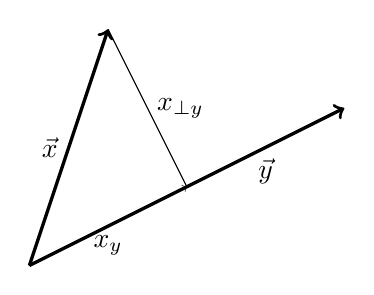
\begin{tikzpicture}
\coordinate (0) at (0,0);
\coordinate (A) at (1,3);
\coordinate (B) at (4,2);
\coordinate (C) at (2,1);
\tikzset{->}
\draw[black,very thick] (0) -- (A) node [midway,left]{$\vec{x}$};
\draw[black,very thick] (0) -- (B) node [near end,right,below]{$\vec{y}$};
\draw[black,very thin]  (0) -- (C) node [midway,right,below]{$x_y$};
\draw[-,thin] (A) -- (C) node [midway,right]{$x_{\perp y}$};
\end{tikzpicture}

\end{document}
